\section{Interactive Analysis Process}
\label{sec:analysisprocess}
The complete topic extraction, abnormality estimation, and event examination are tightly integrated into a highly interactive visual analysis workbench, that allows an analyst to observe, supervise, and configure the method in each individual step. The following sections introduce the details of this system and describe how the event detection is embedded within a sophisticated analysis process as shown in Figure~\ref{fig:ad_process}.

\begin{figure}[ht]
	\centering
	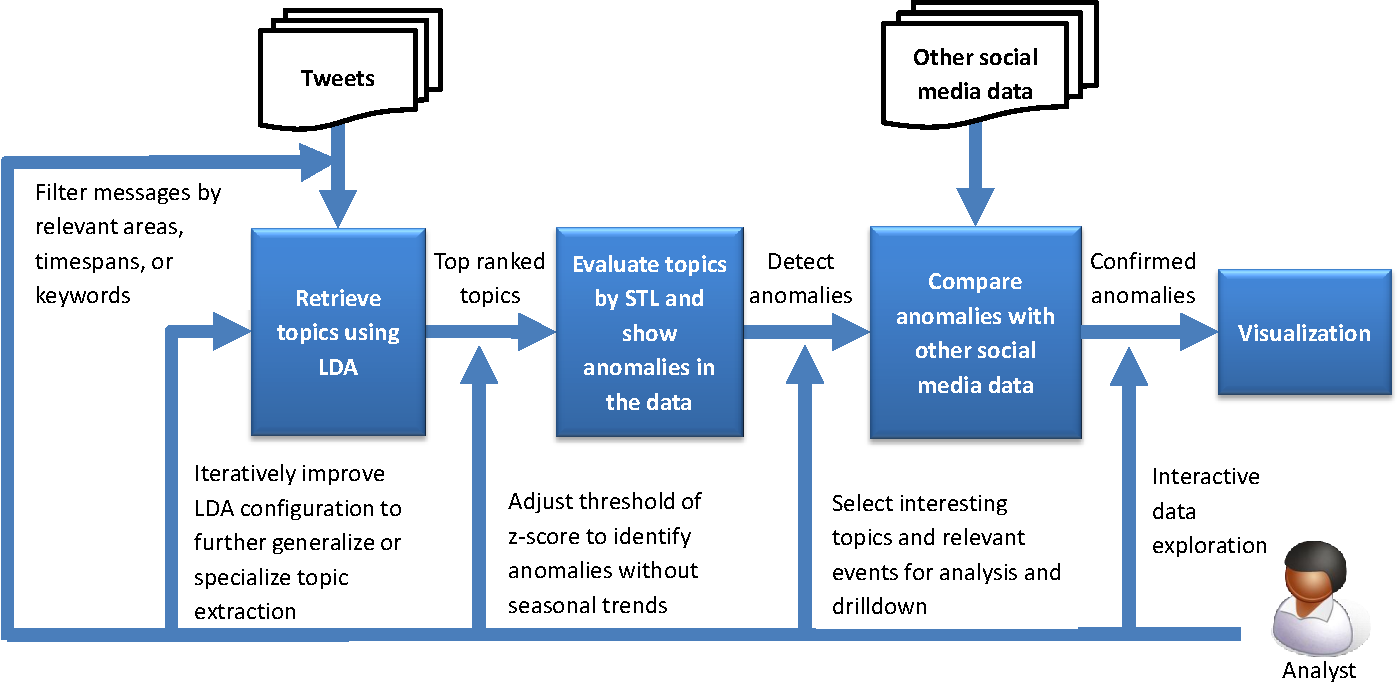
\includegraphics[width=1.0\linewidth]{Overall_Process_crop.pdf}
	\caption{Overview of our iterative analysis scheme for event detection and examination.}
	\label{fig:ad_process}
\end{figure}


\subsection{Social Media Retrieval and Analysis System}
\label{subsec:analysis_system}
Our modular analysis workbench ScatterBlogs was already featured in previous works \cite{Bosch:2011:SGD,Thom:2012:SAD}. 
It proved itself very useful for fundamental tasks like collection, exploration and examination of individual, as well as aggregated, social media messages. The UI of the system is composed of several interconnected views and the main view houses a zoomable openstreetmaps implementation showing message geolocations on a world map. The system features a text search engine and visual content selection tools that can be used to retrieve messages, show spatial and temporal distributions and display textual message contents. Additional visualizations and map overlays provide the analyst with powerful inspection tools, such as a kernel-density heatmap similar to \cite{Maciejewski:2010:VAA}, to show aggregated and normalized message distributions and a movable lens-like exploration tool (called \textquoteleft content lens\textquoteright) that aggregates keyterm frequencies in selected map areas \cite{Bosch:2011:SGD}. To indicate spatiotemporal anomalies in the message set, the system features a mechanism to detect spatiotemporal clusters of similar term usage, and suspicious message clusters can be represented as Tag Clouds on the map \cite{Thom:2012:SAD}. For the real-time collection of messages using the Twitter Streaming API the system features a scalable extraction and preprocessing component. This component was used to collect Twitter messages since August 2011 and it currently processes up to 20 Million messages per day, including the almost complete volume of up to 4 million messages that come with precise geolocation information.

\subsection{Visual Topic Exploration and Event Evaluation}
Results from the topic retrieval and event detection as described in Section~\ref{sec:social_analytics} can be iteratively refined by means of visual result presentation and interactive parameter steering. Both, the final result of event detection as well as intermediary findings during data filtering and topic extraction can be used by the analyst to adjust the process in order to identify interesting topics and keyterms as well as relevant map areas and timespans for a given analysis task. New insights can be generated on each of four individual analysis layers which, in conclusion form an iterative analysis loop from data filtering to result visualization:
\begin{itemize}
	\item \textbf{Spatiotemporal Data Filtering:} The analyst selects an initial spatiotemporal context of Twitter messages to be represented in the visualization and to serve as a basis for analysis. 
He can do so by using textual as well as spatiotemporal query and filter mechanisms that load the relevant base message set from a larger database into active memory. 
The analyst can further filter the base set and remove unimportant parts by using a time-slider, depicting temporal message densities, or polygon and brush selection tools.
% shortened because is prior art
%To filter this base set and to remove unimportant parts, the analyst is provided with an hierarchical time-slider, allowing individual selection of days, hours and minutes. 
%This slider also shows message densities as histograms along the three temporal axis in order to identify high message concentrations. 
%At the same time, polygon and brush selection tools can be applied for spatial filtering.
Using these tools the analyst can gain an initial impression of the spatial and temporal distribution and location of messages that could be relevant for his analysis task.
	\item \textbf{LDA Topic Examination:} In the subsequent step the analyst can choose to start the topic extraction either on the whole analysis context or on some subset of selected messages. At this stage he can utilize the configuration parameters of LDA extraction to interactively explore available topics by generalization and specialization. In this regard the most important parameter is the number of topics that have to be defined for the topic model inference. If the analyst decreases the number using the provided tools, the extracted topics will be more general. If he increases it, they will be more specific and thus candidates for small but possible important events. Once topics are generated from the data they will be presented to the analyst through a list of small tag clouds for each topic. He can now select the topics from the list to see their individual message distribution on the map and the temporal distribution in the time-slider. 
	\item \textbf{STL Evaluation:} Depending on the analyst's choice, the topics can be evaluated and ordered based either on absolute topic frequency or based on abnormality estimates that have been computed using STL. As described in Section~\ref{subsec:filtering}, a valid estimate of abnormality depends on the computation of z-scores from data seven days prior to the observed time frame. Therefore, the STL evaluation will extend the data examination to a range prior to the selected spatiotemporal context, if data is available. Once abnormality is computed for each topic, the topic list will be ordered according to the values and the topics with most outstanding abnormality are highlighted.
	\item \textbf{Crosscheck Validation:} Each selection of messages is accompanied by charts showing the total time series and the remainder components for the selected message set using STL. This is true for spatiotemporal selections as well as for selections using the LDA topic list. In addition to the geolocated Twitter messages this STL is at the same time performed for data that has been extracted from supplemental services like Flickr and YouTube. Based on the multiple charts the analyst can crosscheck the importance and abnormality of examined events and topics.
\end{itemize}


In our system, the analyst is supposed to iteratively use these means of semi-automated processing, visualization and interaction to refine the selection of messages up to a point where he can begin to examine individual message details.
For this task, he can then utilize tools like the content lens for small scale aggregation or the table view to read the messages textual content.
The application of these tools is shown in Figure~\ref{fig:tagcloud}. Usually the most valuable messages will be reports from local eyewitnesses of an important event or from insiders for a given topic. Thus, to retrieve large quantities of such messages helping to understand an ongoing event or situation will be the final goal of the iterative process. Unusual topics, suspicious keyword distributions and events with high STL abnormality discovered on the repeatedly traversed analysis layers can guide the analysis from a very broad and general overview to very specific topics and a relatively small message set suitable for detailed examination.

\begin{figure}[htb]
	\centering
	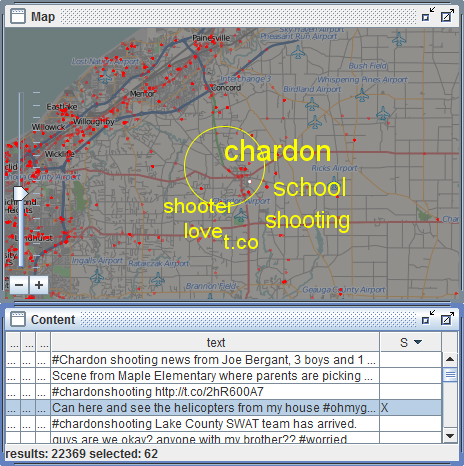
\includegraphics[width=0.6\linewidth]{images/content_investigation}
	\caption{Examining the location of the Chardon high school shooting with a text aggregating content lens.}
	\label{fig:tagcloud}
\end{figure}
